\chapter{PROSES DAN PENGEMBANGAN DESAIN}

% Bab Studi Literatur digunakan untuk mendeskripsikan kajian literatur yang terkait dengan persoalan tugas akhir. Tujuan studi literatur adalah:

% \begin{enumerate}
%     \item menunjukkan kepada pembaca adanya gap seperti pada rumusan masalah yang memang belum terselesaikan,
%     \item memberikan pemahaman yang secukupnya kepada pembaca tentang teori atau pekerjaan terkait yang terkait langsung dengan penyelesaian persoalan, serta
%     \item menyampaikan informasi apa saja yang sudah ditulis/dilaporkan oleh pihak lain (peneliti/Tugas Akhir/Tesis) tentang hasil penelitian/pekerjaan mereka yang sama atau mirip kaitannya dengan persoalan tugas akhir.
% \end{enumerate}

\section{Tinjauan Pustaka}
% Resource Allocator (VideoStorm)
% VAP (DDS)
% Tools (gRPC, tc, python, linux)

    \subsection{Resource Allocator}
    Kehadiran sebuah \textit{resource allocator} merupakan hal yang sangat krusial pada keberlangsungan sistem \textit{edge computing}. Keterbatasan sumber daya komputasi merupakan motivasi
    utama dibalik kebutuhan sistem ini. Sumber daya komputasi harus secara cerdas dan tepat dialokasikan sesuai dengan kebutuhan perangkat \textit{edge} 
    sehingga tidak terdapat \textit{backlog} yang dapat menurukan performansi \citep{edgeComp2}.
    Sumber daya komputasi yang bisa dialokasikan berupa \gls{cpu}, \gls{gpu}, \textit{bandwidth}, \textit{memory}, dan \textit{storage} \citep{edgeCompDis}.

    Beberapa peneliti sudah mengajukan sistem \textit{resource allocator}, diantaranya adalah VideoStorm \citep{videostorm}, \gls{jcab} \citep{jcab}, dan AutoML \textit{for \gls{vap}} \citep{automl}.
    \gls{jcab} melakukan alokasi berdasarkan \textit{bandwidth} dan model \gls{cnn}, artinya pada suatu sistem, terdapat beberapa model yang di-\textit{deploy} berdasarkan resolusi video masukan. 
    Tiap kumpulan video akan didistribusikan pada model \gls{cnn} yang berbeda-beda mengikuti konfigurasi video yang sudah ditentukan sebelumnya.

    Sementara AutoML \textit{for \gls{vap}} adalah sebuah \textit{framework} AutoML yang sengaja dibuat untuk memilih konfigurasi yang teroptimasi untuk \gls{vap} dan pembuatan model \gls{cnn}. VideoStorm, di lain sisi
    adalah sebuah \textit{resource allocator} yang melakukan alokasi terhadap \textit{bandwidth}. Cara kerja VideoStorm adalah pertama-tama kamera-kamera akan mengirimkan video kepada server.
    Lalu pada suatu periode tertentu, VideoStorm akan melakukan alokasi \textit{bandwidth} dengan menganalisis hasil dari beberapa detik sebelumnya dan menentukan \textit{bandwidth} yang sesuai dengan kebutuhannya.
    
    \subsection{Video Analytics Application}

    Faktor utama keberhasilan sebuah sistem \textit{Video Analytics} selaras dengan \textit{Video Analytics Application} (\gls{vap}) yang digunakan. Semakin cerdas \gls{vap}
    maka akan semakin baik performansi yang dihasilkan oleh sistem. \citep{killer} mengatakan bahwa \gls{vap} merupakan sistem yang sangat kompleks jika ingin diterapkan pada jaringan \textit{edge}.
    Hal ini diakibatkan oleh video yang memiliki ukuran data yang relatif besar dan waktu pemrosesan yang cukup lama. Sehingga diperlukan pertimbangan yang sangat matang dalam mendesain sebuah \gls{vap}.

    Sebuah sistem \gls{vap} terdiri dari \textit{client}, \textit{middleware}, dan \textit{server}. \textit{Client} biasanya berupa kamera yang digunakan untuk menangkap video dan melakukan beberapa proses seperti \textit{encoding}
    untuk dikirimkan kepada \textit{server}. \textit{Middleware} adalah sebuah sistem yang menghubungkan \textit{client} dengan \textit{server} yang berfungsi untuk menjamin keberlangsungan transmisi data antar keduanya \citep{middleware}.
    Sementara \textit{server} berguna untuk memproses data seperti melakukan deteksi objek, mengklasifikasikan objek, atau melakukan kegiatan komputasi lainnya.

    Beberapa \gls{vap} sudah diajukan diantaranya adalah \gls{dds} \citep{dds}, AWStream \citep{aws}, Reducto \citep{reducto}, dan Glimpse \citep{glimpse}.
    \gls{dds} adalah sebuah \gls{vap} yang bekerja dengan cara mengirim video menggunakan 2 kali iterasi sehingga dapat diperoleh hasil yang baik. Salah satu persyaratan dalam mendesain \gls{vap}
    adalah \textit{self-adaptability} \citep{chameleon}, hal ini bermakna bahwa \gls{vap} dapat beradaptasi dengan kondisi lingkungannya dengan cara mengubah konfigurasi videonya.

    % Float adalah \textit{container} untuk elemen-elemen dokumen yang tidak dapat dipisah menjadi beberapa halaman. Environment ``table'' dan ``figure'' secara default adalah float. Float berguna untuk memudahkan peletakan objek yang tidak cukup jika diletakkan di halaman sekarang. Peletakan float diatur oleh \LaTeX\ dan pengguna sebaiknya memberikan keleluasaan kepada \LaTeX\ agar dapat mengatur peletakan dengan baik. 
    
    \subsection{Traffic Control}
    \textit{Traffic control} atau lebih dikenal dengan tc adalah sebuah \textit{tools} pada linux yang dapat digunakan untuk memegang kendali atas trafik pada kernel linux \citep{tc}.
    Beberapa fungsi utama dari tc adalah \textit{SHAPING}, \textit{SCHEDULING}, \textit{POLICING}, dan \textit{DROPPING}.

    Salah satu \textit{use-case} yang paling sering digunakan yakni tc akan digunakan sebagai alat yang dapat mengontrol transmisi dari sebuah \textit{interface} jaringan,
    salah satunya adalah untuk menurunkan atau mengelompokan  \textit{ingress bandwidth} ke beberapa \textit{virtual interface} sehingga kelakuannya dapat dikontrol.

    \subsection{gRPC}
    gRPC adalah sebuah \textit{framework} RPC atau \textit{Remote Procedure Call} \textit{open source} universal yang dikembangkan oleh Google \citep{grpc}.
    gRPC digunakan sebagai \textit{tools} penghubung antar perangkat atau perangkat dengan \textit{server} yang dapat dicopot pasang secara mudah.
    % \includesvg{./resources/grpc.svg}
    \begin{figure}[tbh]
        \centering
        \includesvg[scale=0.75]{./resources/grpc.svg}
        \caption{Use-Case gRPC \citep{grpc}}\label{fig:gRPC}
    \end{figure}

    gRPC adalah \textit{framework} RPC yang universal, hal ini bermakna bahwa gRPC mendukung komunikasi data menggunakan bahasa pemrograman yang berbeda
    seperti yang ditunjukan pada Gambar \ref{fig:gRPC}. gRPC menggunakan \textit{Protocol Buffers} atau protobuf sebagai struktur data pada pesan yang dikirimkan,
    secara sekilas, protobuf mirip seperti JSON, namun protobuf universal, lebih ringan, dan lebih cepat dari segi performansi.

    gRPC mendukung berbagai macam jenis komunikasi yakni
    \begin{enumerate}
        \item \textit{Unary RPC} yaitu \textit{client} akan mengirimkan sebuah \textit{request} dan \textit{server} akan mengirimkan sebuah respon. Pada komunikasi ini, hanya \textit{server} yang dapat mengirimkan respon, tidak berlaku sebaliknya
        \item \textit{Server streaming RPC} yaitu \textit{client} akan mengirimkan sebuah \textit{request} dan \textit{server} akan mengirimkan respon yang tak henti hingga pesannya selesai.
        \item \textit{Client streaming RPC} yaitu kebalikannya dari \textit{Server streaming RPC}, yakni \textit{server} yang akan melakukan \textit{request} dan \textit{client} yang akan mengirimkan pesan tak henti.
        \item \textit{Bidirectional streaming RPC} yaitu \textit{client} dan \textit{server} dapat mengirim \textit{request} dan mendapat respon dari satu sama lain
    \end{enumerate}
    % \subsection{Python}
    % \subsection{Linux}
    % \subsubsection{Gambar}
    
    % Float bisa di-\textit{cross reference}. Contohnya Gambar~\ref{fig:contoh_gambar} adalah contoh gambar.

    % \begin{figure}[h]
    %     \centering
    %     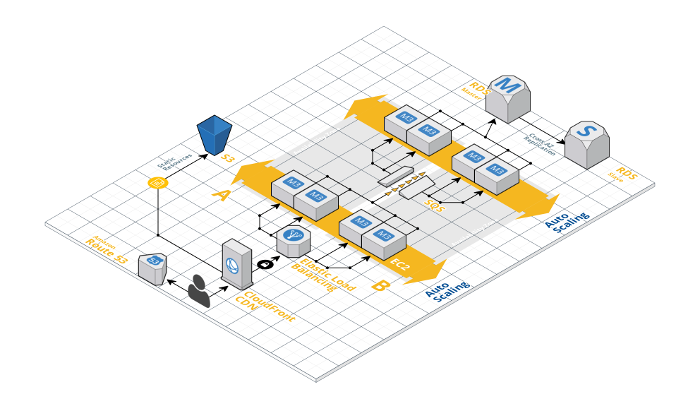
\includegraphics[width=0.8\textwidth]{resources/chapter-2-infrastructure-diagram.png}
    %     \caption{Contoh gambar}
    %     \label{fig:contoh_gambar}
    % \end{figure}

    % \subsubsection{Tabel}

    % Tabel juga merupakan float. Tabel~\ref{table:contoh_tabel} adalah contoh tabel.

    % \begin{table}[htbp]
    %     \small
    %     \centering
    %     \caption{Contoh Tabel}
    %     \label{table:contoh_tabel}
    %     \begin{tabular}{ll}
    %         \toprule
    %         \multicolumn{1}{l}{\textbf{Contoh Judul Kolom}} & \multicolumn{1}{l}{\textbf{Nilai}}\\
    %         \midrule
    %         Besaran 1 & 12 meter          \\
    %         Besaran 2 & $360^\circ$       \\
    %         Besaran 3 & 0,2 meter         \\
    %         Besaran 4 & $1^\circ$         \\
    %         Besaran 5 & 8000 sampel/detik \\
    %         \bottomrule
    %     \end{tabular}
    % \end{table}

    % \subsection{Persamaan Matematika}

    % \blindtext Persamaan~\eqref{eq:contoh_equation} adalah contoh persamaan matematika,

    % \begin{align}
    %     c^2 = a^2 + b^2\,.
    % \label{eq:contoh_equation}
    % \end{align}
    
    % Contoh penggunaan notasi custom,
    
    % \begin{align}
    %     \bayes{x}{y}\,.
    % \label{eq:contoh_equation_custom}
    % \end{align}

\section{Persyaratan Desain}
    \textit{Resource allocator} yang dirancang akan diintegrasikan dengan sebuah \gls{vap} terbaik dari segi performansi yakni \gls{dds}.
    Dengan berbagai macam pertimbangan, sistem yang didesain harus bisa memenuhi rancangan mengikuti objektif sebagai berikut
    \begin{enumerate}
        \item \textit{Resource allocator} bersifat real-time (\textit{Real-time design})
        \item \textit{Resource allocator} harus bisa melakukan tradeoff yang minimal antara bandwidth dan akurasi (\textit{Optimal Trade-off})
        \item \textit{Resource allocator} memiliki harga pengembangan yang minimal (\textit{Minimum Costs})
    \end{enumerate}

    Objektif-objektif yang disebutkan masih bersifat umum. Maka dari itu, akan dilakukan penjabaran dari tiap-tiap objektif dalam bentuk
    pohon subobjektif seperti pada gambar \ref{fig:obj_tree} berikut ini
    % Comment this block if not needed
    \begin{figure}[tbh]
        \centering
        \includesvg[scale=0.35]{./resources/Obj_Tree.svg}
        \caption{Pohon Objektif}\label{fig:obj_tree}
    \end{figure}


    % \begin{center}
    %     \begin{tabular}{|m{9cm}|}
    %         \hline

    %         % (\begin{itemize}
    %         %     \item Objektif 1: \textit{Real-time Design}
    %         % \end{itemize})\\
    %         % Lorem Ipsum \\
    %         \begin{outline}
    %             \1[$\bullet$] Objektif 1: \textit{Real-time Design}
    %                 \2[$\circ$] Subojektif 1: Latensi Minimum
    %             \1[$\bullet$] Objektif 2: \textit{Trade-off} optimal 
    %                 \2[$\circ$] Subobjektif 2: Alokasi \textit{bandwidth} terhadap akurasi \textit{inference}
    %             \1[$\bullet$] Objektif 3: Harga minimum 
    %                 \2[$\circ$] Subobjektif 3: Sistem operasi yang bersifat \textit{open source}
    %         \end{outline}\\
    %         \hline
    %     \end{tabular}
    % \end{center}

    Dari subobjektif tersebut, dibutuhkan suatu batasan agar desain memiliki sebuah acuan yang pasti dan batasan ini tidak bisa dilanggar.
    Batasan atau \textit{constraint} yang ditentukan adalah seperti yang dapat ditemukan pada tabel \ref{tab:constraint}

    \begin{center}
        \begin{table}
            \caption{Tabel \textit{Constraint} pada Subobjektif}\label{tab:constraint}
            \begin{tabular}{|m{12cm}|}
                \hline\\
                \begin{outline}
                    \1[$\bullet$] \textbf{Objektif 1}: \textit{Real-time Design}
                    \2[$\circ$] \textbf{Subobjektif 1}: Latensi Minimum
                    \3[$\circledcirc$] \textbf{\textit{Constraint}}: Latensi E2E tidak melebihi 1 detik
                    \1[$\bullet$] \textbf{Objektif 2}: \textit{Trade-off} optimal 
                    \2[$\circ$] \textbf{Subobjektif 2}: Alokasi \textit{bandwidth} terhadap akurasi \textit{inference}
                    \3[$\circledcirc$] \textbf{\textit{Constraint}}: Ketersediaan \textit{bandwidth} yang terbatas untuk klien sumber video
                    \1[$\bullet$] \textbf{Objektif 3}: Harga minimum 
                    \2[$\circ$] \textbf{Subobjektif 3}: Sistem operasi yang bersifat \textit{open source}
                    \3[$\circledcirc$] \textbf{\textit{Constraint}}: Harus menggunakan sistem operasi Linux
                \end{outline}\\
                \hline
            \end{tabular}
        \end{table}
    \end{center}

%     Fungsi bermanfaat untuk mencapai objektif atau subobjektif melalui komponen-komponen desain yang konkrit. Hal ini dilakukan dengan menentukan persyaratan fungsional desain berdasarkan persyaratan objektif/subobjektif dan constraint. 
% Dari persyaratan fungsional, selanjutnya diidentifikasi fungsi-fungsi untuk memenuhi persyaratan tersebut. Dengan demikian, fungsi dapat dipandang sebagai sebuah sistem, yang menerima sinyal masukan lalu memprosesnya sehingga dihasilkan sinyal luaran. Untuk merealisasikan fungsi yang kompleks, kita dapat membagi sistem menjadi beberapa subsistem yang lebih sederhana.
    Berdasarkan Subobjektif dan \textit{constraint} yang sudah diturunkan, diperlukan sebuah fungsi yang bertujuan untuk memenuhi persyaratan subobjektif dan \textit{constraint}.
    Selanjutnya akan diturunkan persyaratan fungsional dan identifikasi fungsi-fungsi yang dipandang akan menjadi sebuah sistem seperti pada tabel \ref{tab:functional}

    \begin{center}
        \begin{table}
            \caption{Tabel Persyaratan Fungsional dan Fungsi}\label{tab:functional}
            \begin{tabular}{|m{4.5cm}|m{4cm}|m{3.5cm}|}
                \hline
                \thead{Subobjektif dan \textit{Constraint}} &  \thead{Persyaratan Fungsional} & \thead{Fungsi} \\
                \hline
                \begin{outline}
                    \0 \textbf{Subobjektif 1}: Latensi Minimum
                    \1[] \textbf{\textit{Constraint}}: Latensi E2E (\textit{end-to-end}) tidak melebihi 1 detik
                    \0 \textbf{Subobjektif 2}: Alokasi \textit{bandwidth} terhadap akurasi \textit{inference}
                    \1[] \textbf{\textit{Constraint}}: Ketersediaan \textit{bandwidth} yang terbatas untuk klien \gls{vap}
                    \0 \textbf{Subobjektif 3}: Sistem operasi yang bersifat \textit{open source}
                    \1[] \textbf{\textit{Constraint}}: Harus menggunakan sistem operasi Linux
                \end{outline} & 
                \begin{enumerate}
                    \item Latensi E2E (\textit{end-to-end})
                    pada sistem tidak lebih
                    dari 1 detik untuk
                    menghindari terjadinya
                    \textit{backlog} saat pengukuran \textit{overhead}
                    \item Kebutuhan alokasi efisien
                    terhadap ketersediaan
                    \textit{bandwidth} yang terbatas
                    untuk mencapai nilai
                    akurasi inferensi yang
                    terbaik
                    \item Linux digunakan sebagai
                    sistem operasi karena
                    beberapa program hanya
                    dapat berjalan pada sistem operasi
                    tersebut (contohnya: TC)
                \end{enumerate} & \begin{enumerate}
                    \item Mendesain sistem \textit{multiprocessing}
                    \item Menjalankan algoritma komputasi
                    \item Menggunakan Linux beserta \textit{tools}-nya
                \end{enumerate} \\
                \hline
            \end{tabular}
        \end{table}
    \end{center}

    % Insert flow chart here
    \begin{figure}[tbh]
        \centering
        \includesvg[scale=0.8]{./resources/Resource_Allocator.svg}
        \caption{Tingkah Laku Sistem}\label{fig:resource_alloc}
    \end{figure}

\section{Konsep Desain}

    Metrik Objektif
    \begin{center}
        \begin{table}
            \caption{Tabel Persyaratan Fungsional dan Fungsi}\label{tab:functional}
            \begin{tabular}{|m{3cm}|m{3.5cm}|m{5.5cm}|}
                \hline
                \thead{Subobjektif} &  \thead{Metrik Pengukuran} & \thead{Syarat Pemenuhan} \\
                \hline
                Latensi Minimum & Tidak lebih dari 1 detik & \begin{outline}
                    \0 Standard ETSI TR 101 329 V2.1.1; Telecommunications and Internet Protocol Harmonization Over Networks (TIPHON): General aspects of Quality of Service (QoS)
                    \vspace{0.8cm}
                    \0 Standard IEEE POSIX.4; Application With Real-time Application
                \end{outline} \\
                \hline
                Alokasi \textit{bandwidth} terhadap akurasi \textit{inference} & Dapat meningkatkan akurasi sebesar 10\% & Minimum 10\% \citep{dds}\\
                \hline
                Sistem operasi yang bersifat \textit{open source} & 40\% biaya digunakan dari total biaya yang dianggarkan & Maksimum 40\% dari total biaya\\
                % \begin{outline}
                %     \0 \textbf{Subobjektif 1}: Latensi Minimum
                %     % \1[] \textbf{\textit{Constraint}}: Latensi E2E (\textit{end-to-end}) tidak melebihi 1 detik
                %     \0 \textbf{Subobjektif 2}: Alokasi \textit{bandwidth} terhadap akurasi \textit{inference}
                %     % \1[] \textbf{\textit{Constraint}}: Ketersediaan \textit{bandwidth} yang terbatas untuk klien \gls{vap}
                %     \0 \textbf{Subobjektif 3}: Sistem operasi yang bersifat \textit{open source}
                %     % \1[] \textbf{\textit{Constraint}}: Harus menggunakan sistem operasi Linux
                % \end{outline} & 
                % \begin{outline}
                %     \item Tidak lebih dari 1 detik
                %     \item Dapat meningkatkan akurasi sebesar 10\%
                %     \item 40\% biaya digunakan dari total biaya yang dianggarkan
                % \end{outline} & \begin{outline}
                %     \item Mendesain sistem \textit{multiprocessing}
                %     \item Menjalankan algoritma komputasi
                %     \item Menggunakan Linux beserta \textit{tools}-nya
                % \end{outline} \\
                \hline
            \end{tabular}
        \end{table}
    \end{center}

    Pengukuran Constraint
    \begin{center}
        \begin{table}
            \caption{Tabel Persyaratan Fungsional dan Fungsi}\label{tab:functional}
            \begin{tabular}{|m{4.5cm}|m{4cm}|m{3.5cm}|}
                \hline
                \thead{Subobjektif dan \textit{Constraint}} &  \thead{Cara Pengukuran} & \thead{Syarat Pemenuhan} \\
                \hline
                \begin{outline}
                \0 \textbf{Subobjektif}: Alokasi \textit{bandwidth} terhadap akurasi inferensi 
                \0 \textbf{\textit{Constraint:}} Ketersediaan \textit{bandwidth} yang terbatas untuk klien sumber video
                \end{outline} & Melakukan pengukuran penambahan akurasi menggunakan beberapa DDS pada bandwidth yang sama & Minimum 10\%
                (referensi: https://dl.acm.org/doi/pdf/10.1145/3387514.3405887) \\
                % \begin{outline}
                %     \0 \textbf{Subobjektif 1}: Latensi Minimum
                %     % \1[] \textbf{\textit{Constraint}}: Latensi E2E (\textit{end-to-end}) tidak melebihi 1 detik
                %     \0 \textbf{Subobjektif 2}: Alokasi \textit{bandwidth} terhadap akurasi \textit{inference}
                %     % \1[] \textbf{\textit{Constraint}}: Ketersediaan \textit{bandwidth} yang terbatas untuk klien \gls{vap}
                %     \0 \textbf{Subobjektif 3}: Sistem operasi yang bersifat \textit{open source}
                %     % \1[] \textbf{\textit{Constraint}}: Harus menggunakan sistem operasi Linux
                % \end{outline} & 
                % \begin{outline}
                %     \item Tidak lebih dari 1 detik
                %     \item Dapat meningkatkan akurasi sebesar 10\%
                %     \item 40\% biaya digunakan dari total biaya yang dianggarkan
                % \end{outline} & \begin{outline}
                %     \item Mendesain sistem \textit{multiprocessing}
                %     \item Menjalankan algoritma komputasi
                %     \item Menggunakan Linux beserta \textit{tools}-nya
                % \end{outline} \\
                \hline
            \end{tabular}
        \end{table}
    \end{center}

\section{Pengembangan Desain}
    Pada hakikatnya, \textit{resource allocator} adalah sebuah perangkat lunak yang bersifat general dan ringan, artinya sistem harus dapat berjalan pada sistem manapun
    dan dapat melakukan komputasi secara cepat. Dengan demikian, terdapat 2 hal yang patut dipertimbangkan dalam pemilihan desain sistem, yakni bahasa pemrograman dan algoritma komputasi.
    Pemilihan 2 hal tersebut harus dapat memenuhi syarat fungsional yang sebelumnya sudah disebutkan yakni sistem harus dapat berjalan di bawah 1 detik.
    Lebih lanjut mengenai pemilihan bahasa pemrograman dan algoritma komputasi akan dibahas pada bagian berikut ini.
    \subsection{Alternatif Desain Bahasa Pemrograman Subsistem \textit{Resource Allocator}}
        Pemilihan bahasa pemrograman merupakan hal yang sangat krusial terhadap proses desain dan pemilihan \textit{tools} yang digunakan. 
        Beberapa bahasa pemrograman dibuat hanya untuk kasus tertentu. Setelah melakukan beberapa studi literatur, penulis memilih 2 bahasa pemrograman
        yang cocok digunakan pada sistem ini, Yakni Python dan JavaScript.

        Alternatif desain bahasa pemrograman pertama adalah Python, python merupakan sebuah bahasa pemrograman tingkat tinggi, berorientasi objek, dan
        terinterpretasi \citep{python}. Python bersifat \textit{portable}, artinya Python dapat dijalankan pada mesin dan sistem operasi manapun.
        Tidak seperti bahasa lainnya, Python memiliki struktur data yang dinamis, sehingga memudahkan \textit{developer} dalam mengembangkan aplikasi yang membutuhkan waktu
        pengembangan yang cepat. Python memiliki \textit{scientific library} yang sangat beragam dan luas, dengan demikian Python banyak digunakan oleh para scientist untuk
        menyelesaikan berbagai macam perhitungan kompleks. Salah satu kelemahan Python adalah bahasa pemrograman ini tidak memiliki kemampuan \textit{multithreading} yang sangat diperlukan
        dalam melakukan komputasi paralel. Sebagai gantinya, Python menggunakan GIL atau \textit{Global Interpreter Lock} yang berguna dalam melakukan \textit{scheduling} antar thread.

        
        % Python dikembangkan pertama kali dikembangkan oleh Guido van
        % Rossum pada tahun 1980an, pada saat ini Python telah berkembang menjadi sebuah bahasa
        % pemrograman yang open source dan telah memiliki komunitasnya tersendiri [18]. Berikut ini
        % adalah keunggulan dan kekurangan dari Bahasa pemrograman Python [19], [20].

            % Keunggulan:
            % \begin{enumerate}
            %     \item Memiliki komunitas yang besar
            %     \item Memiliki banyak pilihan library untuk berbagai macam kebutuhan seperti visualisasi data, machine learning, dan scientific computing
            %     \item Python memiliki efektifitas yang relatif tinggi dibandingkan bahasa pemrograman lainnya, hal ini memungkinkan developer untuk menulis lebih sedikit kode untuk hasil yang sama
            %     \item Portabilitas, hal ini memungkinkan program dapat dijalankan pada sistem operasi yang berbeda-beda tanpa mengubah kode
            %     \item Memiliki use case yang sangat luas (Data Science, Game Development, Machine Learning, Backend Web Application Development, Cybersecurity, dll)
            % \end{enumerate}

            % Kekurangan: 
            % \begin{enumerate}
            %     \item 
            % \end{enumerate}

        Alternatif desain bahasa pemrograman pertama adalah Javascript, JavaScript merupakan sebuah bahasa pemrograman/\textit{scripting} yang digunakan untuk
        mengimplementasikan fitur-fitur kompleks pada sebuah web page seperti peng-update-an
        konten, pengontrolan multimedia, penganimasian gambar, dll \citep{js}. Pada awalnya Javascript hanya
        diperuntukan untuk web page saja, namun pada saat ini Javascript dapat digunakan sebagai
        bahasa yang digunakan pada backend.

        Sama seperti Python, JavaScript adalah bahasa pemrograman yang portabel sehingga bisa dijalankan pada sistem operasi manapun.
        Namun, berbeda dengan Python, JavaScript dapat melakukan \textit{multithreading} sehingga dipandang memiliki kapasitas untuk
        melakukan komputasi yang kompleks \citep{jsDisad}. Beberapa kelemahan JavaScript antara lain adalah bersifat \textit{asynchronous} sehingga
        alur pengkodeannya sukar untuk dipahami dan kurang mendukung untuk \textit{scientific computing}.
        
        % Javascript/node js memiliki kelebihan yang tidak dimiliki oleh python seperti kecepatan dalam
        % memproses data dan kemampuan dalam memproses data yang sangat banyak, Hal ini
        % memenuhi persyaratan fungsional resource allocator, namun kurangnya library untuk scientific
        % computing membuat Javascript kurang cocok digunakan dalam pengembangan resource
        % allocator.

    \subsection{Alternatif Desain Algoritma Komputasi Subsistem \textit{Resource Allocator}}
        Sebuah sistem yang \textit{realtime} tidak akan terwujud tanpa adanya algoritma yang efisien dan kencang. 
        Berikut adalah beberapa alternatif algoritma komputasi untuk mengalokasikan besaran \textit{bandwidth}
        yakni \textit{offline learning} dan \textit{online learning}.

        % Offline Learning
        Offline learning adalah sebuah teknik pembelajaran yang dilakukan oleh sebuah model machine
        learning atau decision maker yang biasa dikenal sebagai batch training. Sebelum melakukan
        pembelajaran, sistem akan mengumpulkan data terlebih dahulu, setelahnya model akan
        dilakukan training dengan menggunakan data tersebut. Dalam kasus lain, offline learning akan
        menghasilkan nilai weight yang seragam pada setiap decision pada data yang akan datang \citep{offlineOnline}.
        Offline learning memiliki banyak kelebihan yakni waktu training yang relatif cepat dan
        kompleksitas yang kecil sehingga dapat memenuhi persyaratan fungsional real-time processing
        pada resource allocator. Selain itu, karena proses training berlangsung dengan sangat singkat, maka tidak ada resource yang perlu dikorbankan. 
        Namun, mode pembelajaran ini tidak terlalu bersifat adaptif, artinya ketika terjadi perubahan pola video,
        decision maker tidak akan menyadari hal itu hingga waktu training selanjutnya. Sehingga dapat dikatakan bahwa 
        offline learning cocok diterapkan pada jenis data yang memiliki pola yang seragam dan tidak cepat berubah.

        % Online Learning
        Sementara itu, Online learning adalah teknik pembelajaran yang merupakan kebalikan dari offline learning.
        Pada online learning, data tidak dikumpulkan terlebih dahulu, namun data yang masuk akan di-training dengan mempertimbangkan model sebelumnya, hal
        ini akan terus berlangsung hingga program selesai. Alhasil besarnya weight pada tiap iterasi
        akan berbeda \citep{online}. Secara umum, online learning bersifat adaptif, terkait hal sebelumnya, hal ini berarti bahwa online learning 
        tahan terhadap data yang memiliki perubahan pola yang cepat dan beragam. Namun terdapat beberapa hal yang dikorbankan, salah satunya adalah kompleksitas
        dan penggunaan resource. Karena proses pembelajaran akan terjadi selama terus menerus, hal ini mengakibatkan kompleksitas algoritma yang tinggi
        memiliki kompleksitas yang lebih tinggi. Selain itu, proses pembelajaran tentunya akan menggunakan resource dan hal ini mengakibatkan server perlu 
        mendedikasikan sebagian resourcenya untuk keberlangsungan pembalajaran.

        
    \subsection{Pemilihan Desain Subsistem \textit{Resource Allocator}}
        Pada bagian ini akan didiskusikan alternatif pemilihan desain bahasa pemrograman dan algoritma komputasi yang sesuai dengan spesifikasi \textit{resource allocator}.

        \begin{table}[tbh]
            \begin{center}
                \caption{Tabel Pemilihan Bahasa Pemrograman}\label{tab:pythonOrJs}
                \begin{tabular}{|c|c|c|}
                    \hline
                    \thead{Spesifikasi} & \thead{Python} & \thead{JavaScript}\\
                    \hline
                    \textit{Cross Platform} & \ding{51} & \ding{51}\\
                    \hline 
                    \textit{Easy Implementation} & \ding{51} & \ding{55}\\
                    \hline
                    \textit{Multithreading} & \ding{55} & \ding{51}\\
                    \hline 
                    \textit{Datascience \& Scientific Computing Friendly} & \ding{51} & \ding{55}\\
                    \hline
                \end{tabular}
            \end{center}
        \end{table}

        Secara ringkas, perbandingan antara bahasa pemrograman Python dan JavaScript adalah seperti tertera pada tabel \ref{tab:pythonOrJs}. Python memenuhi 3 dari 4 persyaratan yang dikehendaki dan
        JavaScript memenuhi 2 dari 4 persyaratan yang dikehendaki.
        Dari hal tersebut, diketahui bahwa bahasa pemgrograman yang paling banyak memenuhi persyaratan adalah Python. Dengan demikian, bahasa pemrograman yang dipilih adalah Python karena bahasa pemrograman ini mendukung \textit{scientific computing} dan kemudahan bahasa.
        Ketersediaan \textit{scientific computing library} sangat penting karena \textit{resource allocator} yang diajukan menggunakan algoritma \textit{linear programming} untuk proses optimasi
        yang mana hal tersebut sangat krusial pada resource allocator yang menggunakan linear programming dalam pengalokasian \textit{bandwidth} nya.
        
        \begin{table}[tbh]
            \begin{center}
                \caption{Tabel Pemilihan Algoritma Komputasi}\label{tab:onlineOrOffline}
                \begin{tabular}{|c|c|c|}
                    \hline
                    \thead{Spesifikasi} & \thead{Online Learning} & \thead{Offline Learning}\\
                    \hline
                    \textit{Computational Efficient} & \ding{55} & \ding{51}\\
                    \hline 
                    \textit{Low Complexity} & \ding{55} & \ding{51}\\
                    \hline
                    \textit{Resource Offloading (\ding{51} means bad)} & \ding{51} & \ding{55}\\
                    \hline 
                    \textit{Content Pattern-Independent} & \ding{51} & \ding{55}\\
                    \hline
                \end{tabular}
            \end{center}
        \end{table}

        Secara ringkas, perbandingan antara Offline Learning dan Online Learning adalah seperti pada tabel \ref{tab:onlineOrOffline}. Offline learning memenuhi 3 dari 4 persyaratan yang dikehendaki dan
        online learning hanya memenuhi 1 dari 4 persyaratan yang dikehendaki. Dari informasi tersebut, diketahui bahwa metode algoritma komputasi yang 
        paling banyak memenuhi persyaratan adalah offline learning. Dengan demikian, alternatif desain algoritma komputasi yang dipilih dalam perancangan \textit{resource allocator} adalah offline learning.
        Kompleksitas yang rendah dan tidak terdapatnya \textit{resource offloading} sangat diperlukan keberedaannya pada \textit{edge computing} karena keterbatasan sumber daya komputasi.
        Dengan demikian, \textit{resource allocator} akan didesain menggunakan bahasa pemrograman Python dan metode algoritma komputasi offline learning.
        % Dengan Demikian, metode algoritma komputasi yang akan digunakan pada \textit{resource allocator} adalah Offline Learning

